%!Mode:: "TeX:UTF-8"
%!TEX encoding=UTF-8 Unicode
\documentclass[UTF8,11pt,colorlinks,aspectratio=43]{beamer}%aspectratio=169 %169宽屏 43窄屏[handout]

\setbeamersize{text margin left=.025\paperwidth,text margin right=.025\paperwidth}
\setbeamertemplate{footline}[frame number]
\setbeamertemplate{navigation symbols}{}
\setbeamertemplate{frametitle}[default][center]
\setbeamertemplate{blocks}[rounded]

%%%%%%%%%%%%%%%% 宏包 %%%%%%%%%%%%%%%%
\usepackage[UTF8,heading=false,scheme=plain]{ctex}
\usefonttheme{professionalfonts}%解决Beamer字体冲突
% Common Packages
\usepackage[english]{babel}%断字
\usepackage[toc]{multitoc}%多栏目录
\usepackage{newtxmath} \let\openbox\relax
\usepackage{csquotes}
\usepackage[backend=biber,style=alphabetic]{biblatex}%doi=false,isbn=false,url=false
%\addbibresource{ref.bib}

% Graphics Packages
\usepackage{graphicx}
\graphicspath{{img/}}
\usepackage{tikz}
\usetikzlibrary{cd}
% TikZ Settings
\tikzset{
 commutative diagrams/.cd,
 arrow style=tikz,
 diagrams={>=latex},
 ampersand replacement=\&,
}

% Colors
\definecolor{background}{RGB}{255,255,255}
\definecolor{red}{RGB}{220,50,47}
\definecolor{green}{RGB}{0,128,0}
\definecolor{yellow}{RGB}{181,137,0}
\definecolor{orange}{RGB}{203,75,22}
\definecolor{pink}{RGB}{247,0,94}
\definecolor{cyan}{RGB}{42,161,152}
\definecolor{blue}{RGB}{9,132,227}
\definecolor{lightgreen}{RGB}{199,237,204}
\definecolor{lightyellow}{RGB}{253,246,227}

%%%%%%%%%%%%%% 颜色设置 %%%%%%%%%%%%%%
\setbeamercolor{normal text}{bg=background}
\setbeamercolor{structure}{fg=orange,bg=lightgreen!25}
\setbeamercolor{block body}{bg=lightgreen!7}
\setbeamercolor{block title example}{fg=orange,bg=lightgreen!25}
\setbeamercolor{block body example}{bg=lightgreen!7}

%-------------------------------%
% Hyperref %
%-------------------------------%

\usepackage{hyperref}
\hypersetup{pdfstartview=FitV,bookmarksopenlevel=0,}


%%%%%%%%%%%%% 标题 %%%%%%%%%%%%%
\title{Slides}
\author{Xi Li}

\begin{document}
\maketitle

%%%%%%%%%%%% 节前目录 %%%%%%%%%%%
\AtBeginSection[]
{
\frame[shrink]{{Contents}
%\begin{multicols}{2}
\tableofcontents[currentsection,hideallsubsections]
%\end{multicols}
}
\addtocounter{framenumber}{-1} %目录页不计页码
}
\AtBeginSubsection[]
{
\frame[shrink]{{Contents}
\begin{multicols}{2}
\tableofcontents[sectionstyle=show/shaded,subsectionstyle=show/shaded/hide,subsubsectionstyle=hide]
\end{multicols}
}
\addtocounter{framenumber}{-1} %目录页不计页码
}


\begin{frame}\frametitle{Diagram}
\[\begin{tikzcd}[column sep=huge, row sep=huge]
X\times X \ar[r,"f"] \& Y \ar[d,"\alpha"]\\
X \ar[r,"g" swap] \ar[u,"\Delta"] \& Y
\end{tikzcd}\]
\[\alpha(f(\ulcorner g\urcorner,\ulcorner g\urcorner))=g(\ulcorner g\urcorner)=f(\ulcorner g\urcorner,\ulcorner g\urcorner)\]
\begin{center}
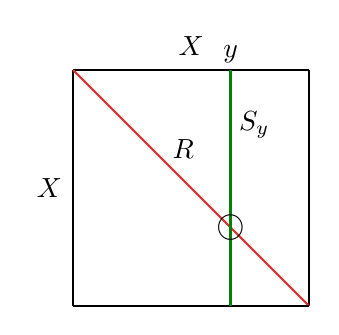
\begin{tikzpicture}
						%\draw [help lines] (0,0) grid (10,5);
						\draw [-,thick] (0,0) -- (0,3);
						\draw [-,thick] (0,3) -- (3,3);
						\draw [-,thick] (3,0) -- (3,3);
						\draw [-,red,thick] (0,3) -- (3,0);
						\draw [-,thick] (0,0) -- (3,0);
						\draw [-,green,thick] (2,0) -- (2,3);
						
						\node at (-0.3,1.5) {$X$};
						\node at (1.5,3.3) {$X$};
						\node at (2,3.2) {$y$};
						\node at (2.3,2.3) {$S_y$};
						\node at (1.4,2) {$R$};
						\node at (2,1) {$\bigcirc$};
\end{tikzpicture}
\end{center}
\end{frame}









%\begin{frame}[allowframebreaks]\frametitle{References}\printbibliography[heading=bibintoc]\end{frame}
\end{document}
